\subsection*{Problema 27}

\textbf{Enunciado:}
Calcular la integral indefinida:
\begin{equation*}
\int \dfrac{3x^2 + x - 2}{(x - 1)(x^2 + 1)} \, dx
\end{equation*}

\textbf{Solución:}
Observamos que el integrando es una función racional propia. 
Utilizamos el método de fracciones parciales. 
Planteamos la descomposición:
\begin{align*}
\dfrac{3x^2 + x - 2}{(x - 1)(x^2 + 1)} &= \dfrac{A}{x - 1} \\
&\quad + \dfrac{Bx + C}{x^2 + 1}
\end{align*}

Multiplicando ambos lados por el denominador común $(x - 1)(x^2 + 1)$, obtenemos:
\begin{align*}
3x^2 + x - 2 &= A(x^2 + 1) \\
&\quad + (Bx + C)(x - 1)
\end{align*}

Para hallar los valores de las constantes, evaluamos en valores convenientes de $x$. 
Si $x = 1$:
\begin{align*}
3(1)^2 + 1 - 2 &= A(1^2 + 1) + 0 \\
2 &= 2A \implies A = 1
\end{align*}

Expandimos y agrupamos términos del lado derecho según las potencias de $x$:
\begin{align*}
3x^2 + x - 2 &= Ax^2 + A + Bx^2 \\
&\quad - Bx + Cx - C \\
&= (A + B)x^2 \\
&\quad + (C - B)x + (A - C)
\end{align*}

Igualando los coeficientes de ambos lados:
\begin{align*}
A + B &= 3 \\
C - B &= 1 \\
A - C &= -2
\end{align*}

Como $A = 1$, de la primera ecuación:
\begin{align*}
1 + B &= 3 \implies B = 2
\end{align*}

De la tercera ecuación:
\begin{align*}
1 - C &= -2 \implies C = 3
\end{align*}

Sustituyendo las constantes $A$, $B$ y $C$ en la descomposición original:
\begin{align*}
\int &\dfrac{3x^2 + x - 2}{(x - 1)(x^2 + 1)} \, dx = \\
&\int \left( \dfrac{1}{x - 1} + \dfrac{2x + 3}{x^2 + 1} \right) dx
\end{align*}

Separamos la integral en tres partes para facilitar la integración directa:
\begin{align*}
&= \int \dfrac{1}{x - 1} \, dx \\
&\quad + \int \dfrac{2x}{x^2 + 1} \, dx + \int \dfrac{3}{x^2 + 1} \, dx
\end{align*}

Integramos cada término aplicando fórmulas estándar (logaritmo natural y arcotangente):
\begin{align*}
&= \ln|x - 1| + \ln(x^2 + 1) \\
&\quad + 3\arctan(x) + C
\end{align*}

Por lo tanto, la solución general de la integral es:
\begin{equation*}
\ln|x - 1| + \ln(x^2 + 1) + 3\arctan(x) + C
\end{equation*}

\begin{figure}[H]
	\centering
	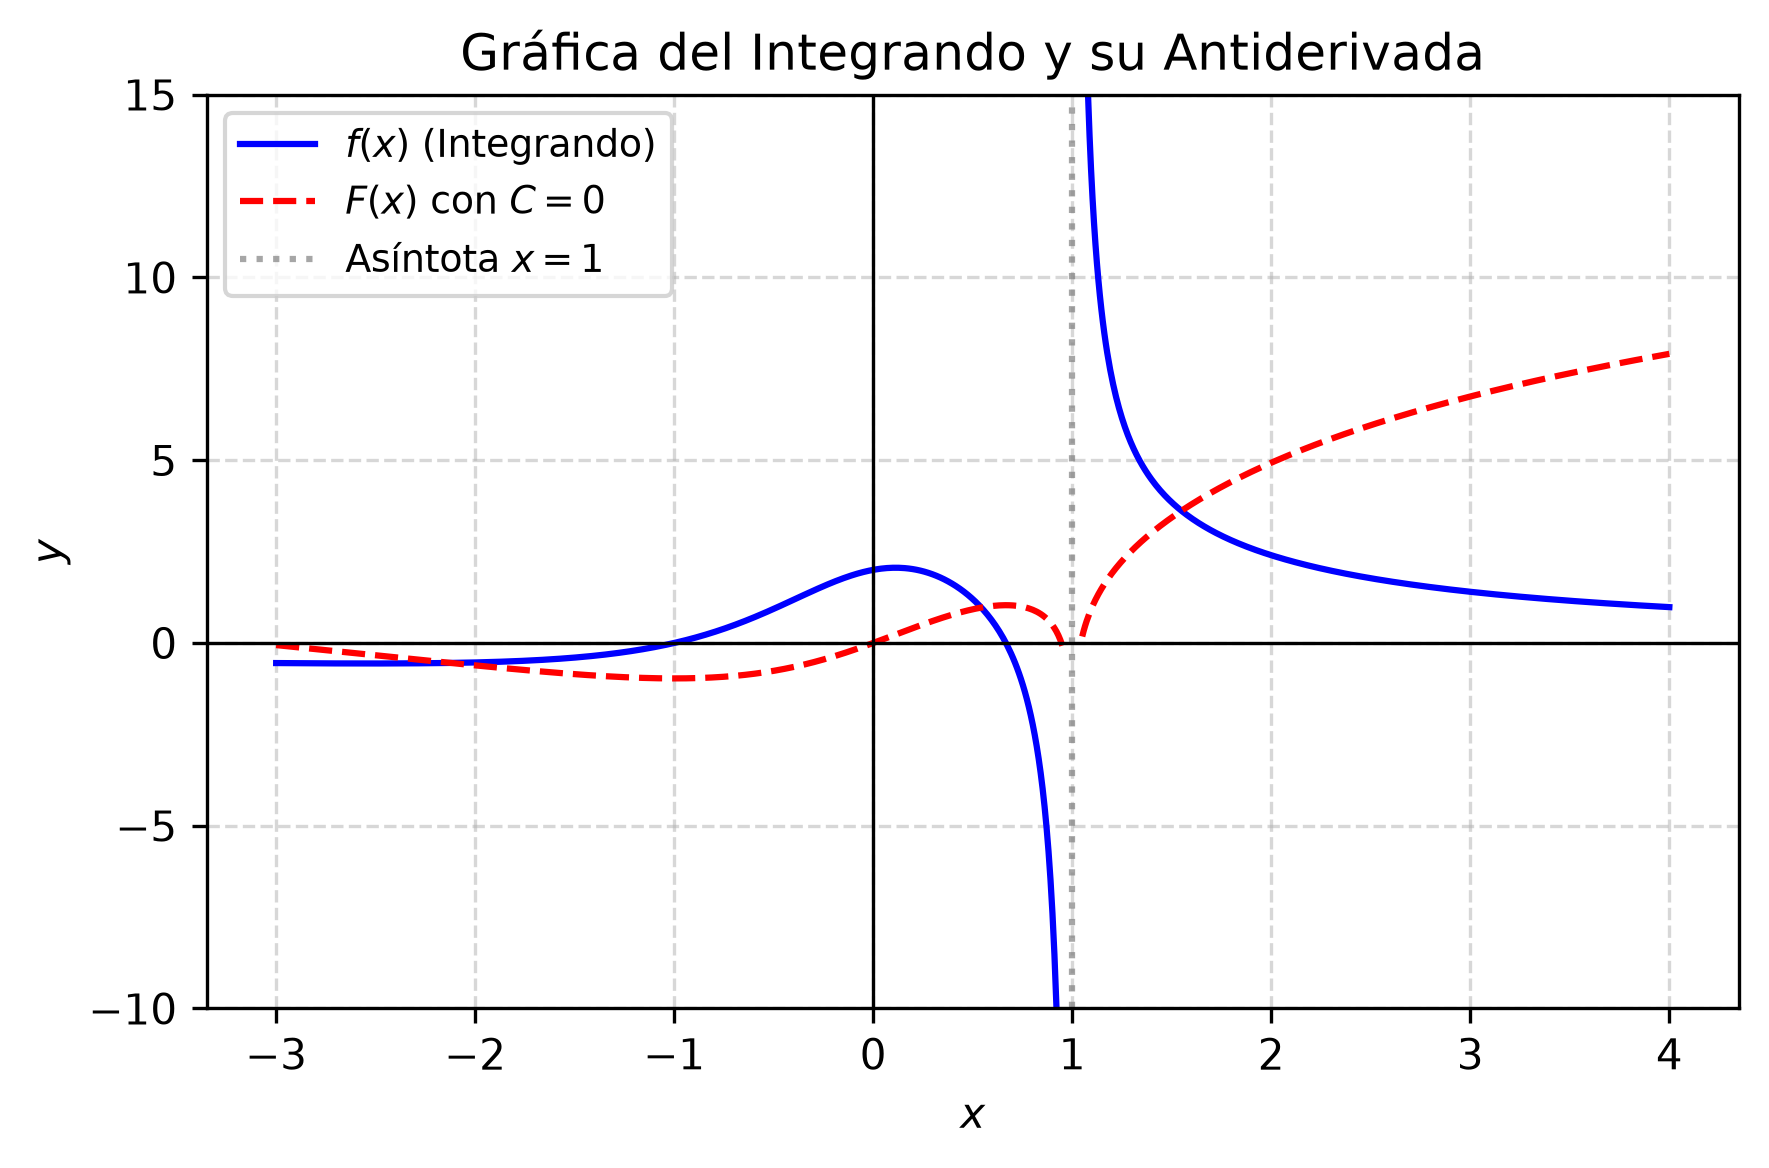
\includegraphics[width=\columnwidth]{semana_03/graficas/SEM03_P27_grafica.png}
	\caption{Representación gráfica de $f(x)$ y su antiderivada $F(x)$ evaluada para la constante de integración $C = 0$ (Problema 27).}
	\label{fig:problema27}
\end{figure}
